\section{Experiments}
\nocite{Kanade2000CK+}\nocite{Lucey2010CK+}

%TODO: describe setup of datasets sued for training and validation.Present results

%\onecolumn

\begin{figure}%[H]
	\centering
	\begin{subfigure}[b]{0.15\textwidth}
		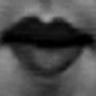
\includegraphics[width=\textwidth]{./img/timeseriesHappy/S026_006_00000001_conew1.png}
		\caption{Neutral-neutral}
		\label{fig:timeseriesHappy:a}
	\end{subfigure}
	%\hspace{\fill}
	\begin{subfigure}[b]{0.15\textwidth}
		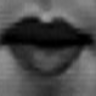
\includegraphics[width=\textwidth]{./img/timeseriesHappy/S026_006_00000002_conew1.png}
		\caption{Neutral-neutral}
		\label{fig:timeseriesHappy:b}
	\end{subfigure}
	%\hspace{\fill}
	\begin{subfigure}[b]{0.15\textwidth}
		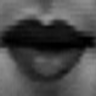
\includegraphics[width=\textwidth]{./img/timeseriesHappy/S026_006_00000003_conew1.png}
		\caption{Neutral-neutral}
		\label{fig:timeseriesHappy:c}
	\end{subfigure}
	%\hspace{\fill}
	\begin{subfigure}[b]{0.15\textwidth}
		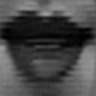
\includegraphics[width=\textwidth]{./img/timeseriesHappy/S026_006_00000004.png}
		\caption{Intermediate-disgust}
		\label{fig:timeseriesHappy:d}
	\end{subfigure}
	%\hspace{\fill}
	\begin{subfigure}[b]{0.15\textwidth}
		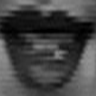
\includegraphics[width=\textwidth]{./img/timeseriesHappy/S026_006_00000005.png}
		\caption{Intermediate-happy}
		\label{fig:timeseriesHappy:e}
	\end{subfigure}
	%\hspace{\fill}
	\begin{subfigure}[b]{0.15\textwidth}
		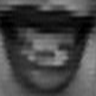
\includegraphics[width=\textwidth]{./img/timeseriesHappy/S026_006_00000006.png}
		\caption{Intermediate-happy}
		\label{fig:timeseriesHappy:f}
	\end{subfigure}
	%\hspace{\fill}
	\begin{subfigure}[b]{0.15\textwidth}
		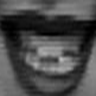
\includegraphics[width=\textwidth]{./img/timeseriesHappy/S026_006_00000007.png}
		\caption{Happy-happy}
		\label{fig:timeseriesHappy:g}
	\end{subfigure}
	%\hspace{\fill}
	\begin{subfigure}[b]{0.15\textwidth}
		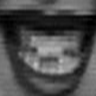
\includegraphics[width=\textwidth]{./img/timeseriesHappy/S026_006_00000008.png}
		\caption{Happy-happy}
		\label{fig:timeseriesHappy:h}
	\end{subfigure}
	%\hspace{\fill}
	\begin{subfigure}[b]{0.15\textwidth}
		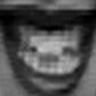
\includegraphics[width=\textwidth]{./img/timeseriesHappy/S026_006_00000009.png}
		\caption{Happy-happy}
		\label{fig:timeseriesHappy:i}
	\end{subfigure}
	%\hspace{\fill}
	\begin{subfigure}[b]{0.15\textwidth}
		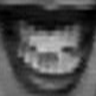
\includegraphics[width=\textwidth]{./img/timeseriesHappy/S026_006_00000010.png}
		\caption{Happy-happy}
		\label{fig:timeseriesHappy:j}
	\end{subfigure}
	%\hspace{\fill}
	\begin{subfigure}[b]{0.15\textwidth}
		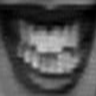
\includegraphics[width=\textwidth]{./img/timeseriesHappy/S026_006_00000011.png}
		\caption{Happy-happy}
		\label{fig:timeseriesHappy:k}
	\end{subfigure}
	%\hspace{\fill}
	\begin{subfigure}[b]{0.15\textwidth}
		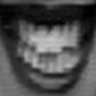
\includegraphics[width=\textwidth]{./img/timeseriesHappy/S026_006_00000012.png}
		\caption{Happy-happy}
		\label{fig:timeseriesHappy:l}
	\end{subfigure}
	%\hspace{\fill}
	\begin{subfigure}[b]{0.15\textwidth}
		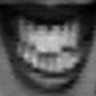
\includegraphics[width=\textwidth]{./img/timeseriesHappy/S026_006_00000013.png}
		\caption{Happy-happy}
		\label{fig:timeseriesHappy:m}
	\end{subfigure}
	\caption[Complete time series of happy mouth patches]{Extracted mouth patch of size 96x96 pixels showing the development of
	the facial expression of happiness from neutral to maximal happy expression.
	Patches \ref{fig:timeseriesHappy:a} to \ref{fig:timeseriesHappy:c} have been
	categorized for training as neutral, patches \ref{fig:timeseriesHappy:d} to
	\ref{fig:timeseriesHappy:g} have been excluded from training and patches
	\ref{fig:timeseriesHappy:e} to \ref{fig:timeseriesHappy:m} have been used as
	positive samples for training happy expressions. Classification identified
	\ref{fig:timeseriesHappy:a} to \ref{fig:timeseriesHappy:c} correctly as
	neutral, \ref{fig:timeseriesHappy:d} was identified as disgust and
	\ref{fig:timeseriesHappy:e} to \ref{fig:timeseriesHappy:m} were classified as
	happy expressions according to table \ref{table:predict_mouth}.}
	\label{fig:timeseriesHappy}
\end{figure}

%\twocolumn

\subsection{Data}
For training a system to recognize facial expression effectively, the dataset should focus on several main expressions including anger, disgust, fear, happiness, sadness and surprise. Moreover, a proper dataset should be composed of faces with kinds of face shapes, colors, facial and scalp hairs from many participants with different genders, ethnic backgrounds and ages.
\\
\\
The dataset this paper adopted is from the Cohn-Kanade Facial Expression Database. The dataset refers to eight emotions including anger, contempt, disgust, fear, happiness, sadness, surprise and neutral expression. There are 5105 images from 123 subjects, who ranged in age from 18 to 30 years. Sixty-five percent are female, eight-five percent are Euro-American and fifteen percent are African-American and Asian. They were observed in an observation room equipped with a chair on which to sit and a camera was located directly in front of the subject. Therefore all images have the uniform background and lighting. The images were digitized into 640*480 or 490 pixel arrays with 8-bit precision for grayscale values and are available in png and jpg.
\\
\\
In the Cohn-Kanade Facial Expression Dataset, subjects performed a series of several facial displays that varied from mild to intense expression for each emotion and images were taken frame by frame. In the mild ones, the emotion is barely noticeable and in the intense ones, it is clearly noticeable. In order to train a robust system, we chose the images mostly with intense expressions which were clearly noticeable. That means all the expressions in our dataset are clearly representing the emotion they belong to and are also distinguishable from other emotions. Figure \ref{fig:dataset images} shows eight examples from eight emotions respectively.


\begin{figure}%[H]
	\centering
	\begin{subfigure}[b]{0.22\textwidth}
		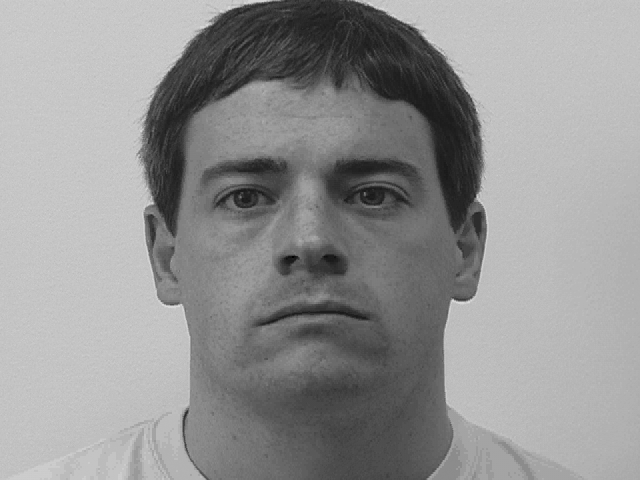
\includegraphics[width=\textwidth]{./img/dataset/neutral.png}
		\caption{neutral}
		\label{fig:dataset:neutral}
	\end{subfigure}
	%\hspace{\fill}
	\begin{subfigure}[b]{0.22\textwidth}
		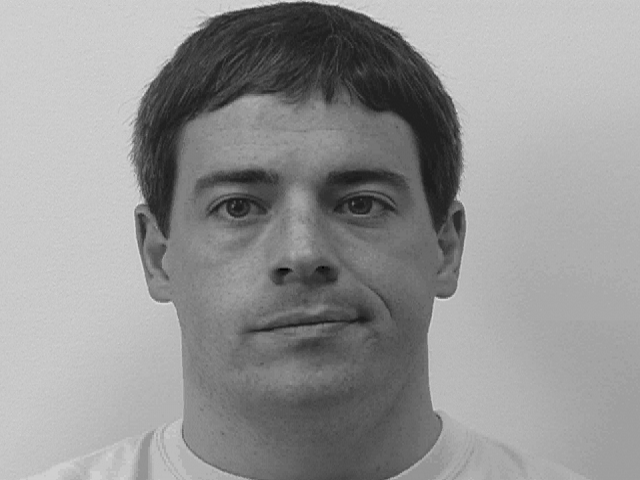
\includegraphics[width=\textwidth]{./img/dataset/contempt.png}
		\caption{contempt}
		\label{fig:dataset:contempt}
	\end{subfigure}
%\hspace{\fill}
	\begin{subfigure}[b]{0.22\textwidth}
		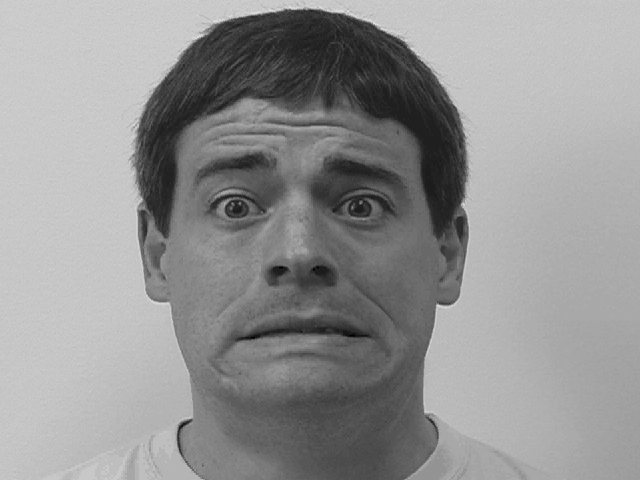
\includegraphics[width=\textwidth]{./img/dataset/fear.png}
		\caption{fear}
		\label{fig:dataset:fear}
	\end{subfigure}
%\hspace{\fill}
	\begin{subfigure}[b]{0.22\textwidth}
		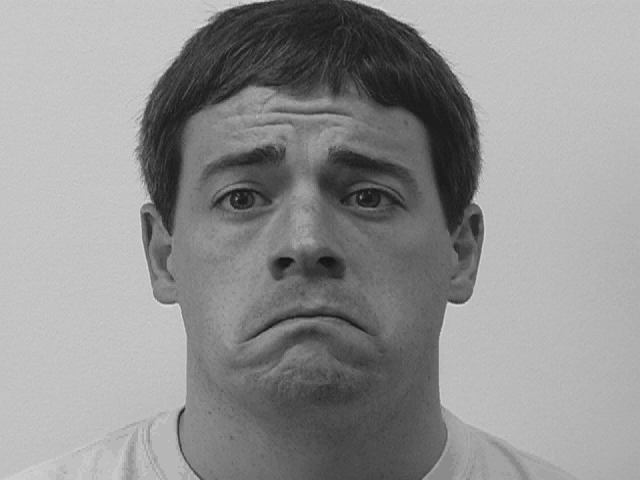
\includegraphics[width=\textwidth]{./img/dataset/sadness.png}
		\caption{sadness}
		\label{fig:dataset:sadness}
	\end{subfigure}
%\hspace{\fill}
	\begin{subfigure}[b]{0.22\textwidth}
		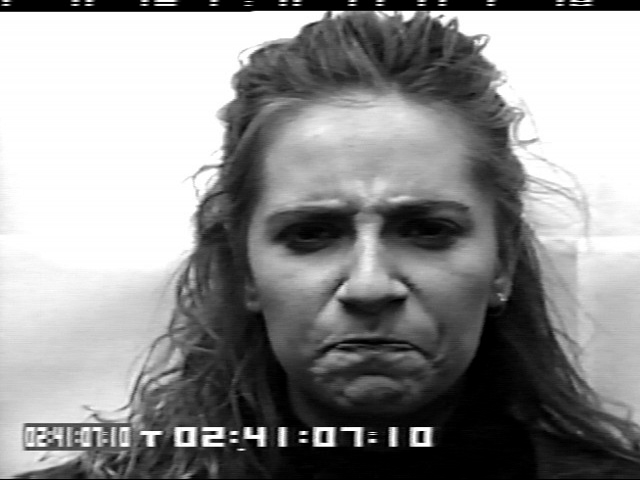
\includegraphics[width=\textwidth]{./img/dataset/angry.png}
		\caption{angry}
		\label{fig:dataset:angry}
	\end{subfigure}
%\hspace{\fill}
	\begin{subfigure}[b]{0.22\textwidth}
		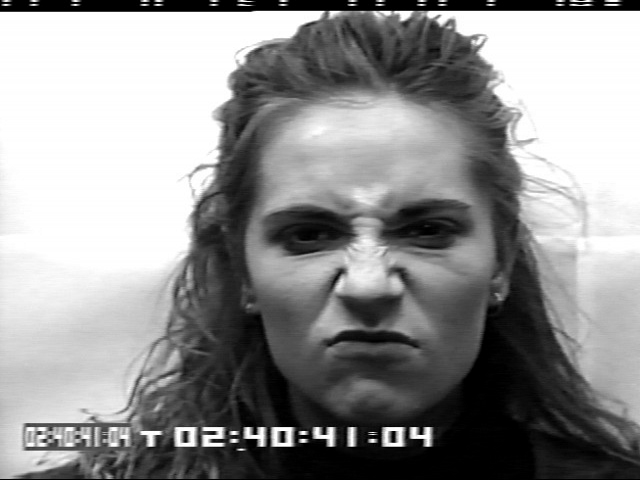
\includegraphics[width=\textwidth]{./img/dataset/disgust.png}
		\caption{disgust}
		\label{fig:dataset:disgust}
	\end{subfigure}
%\hspace{\fill}
	\begin{subfigure}[b]{0.22\textwidth}
		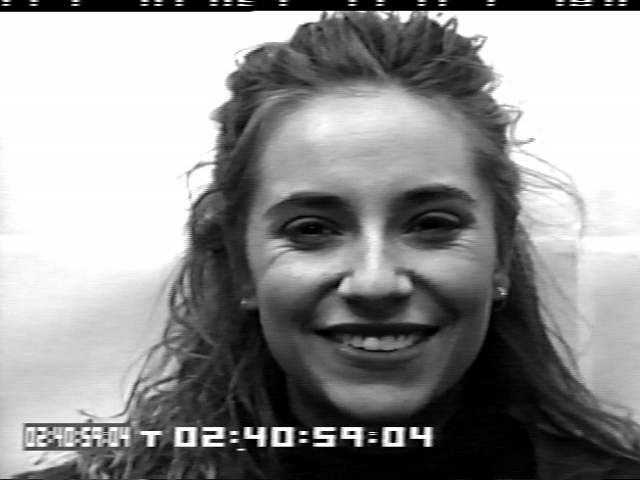
\includegraphics[width=\textwidth]{./img/dataset/happy.png}
		\caption{happy}
		\label{fig:dataset:happy}
	\end{subfigure}
%\hspace{\fill}
	\begin{subfigure}[b]{0.22\textwidth}
		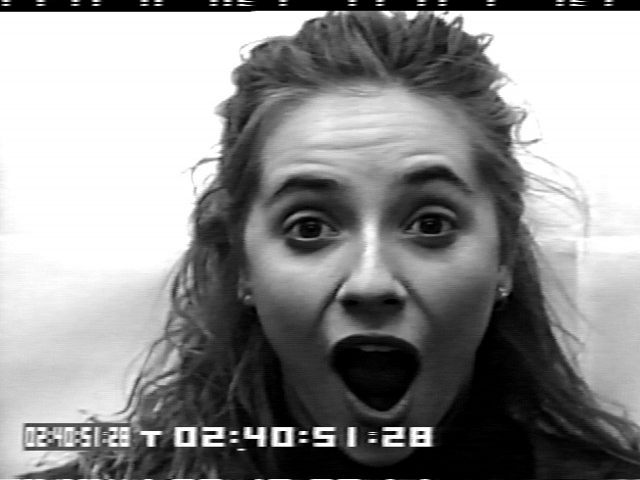
\includegraphics[width=\textwidth]{./img/dataset/surprise.png}
		\caption{surprise}
		\label{fig:dataset:surprise}
	\end{subfigure}
    \caption{Examples of intense facial expressions from two subjects in the dataset}
    \label{fig:dataset images}
\end{figure}

\subsection{Experiment setup}
The experiments were performed doing one versus all classification. The data for each expression is divided into a training and a validation set and an SVM
classifier is calculated based on the training set. The accuracy of the classifiers is then measured on the validation set. It was ensured that images of the same
person are not present in both the training and validation set. The fraction of the data used for the validation set is a configurable parameter, for the
following experiments 75\% of the data was used for the training set and 25\% for the validiation set.

\subsection{Manual Patches}

An image can have multiple discriminating patches. As shown in Figure \ref{fig:manual_patch}, some patches are highly noticeably discriminating such an open mouth and raised eyebrows in "`surprise"' expression or a wrinkled glabella (area between eyes) in "`disgust"' expression. Such patches can be the best approximation of most discriminating patches. Hence, they make a good basis for testing the algorithm.

\begin{figure}
\centering
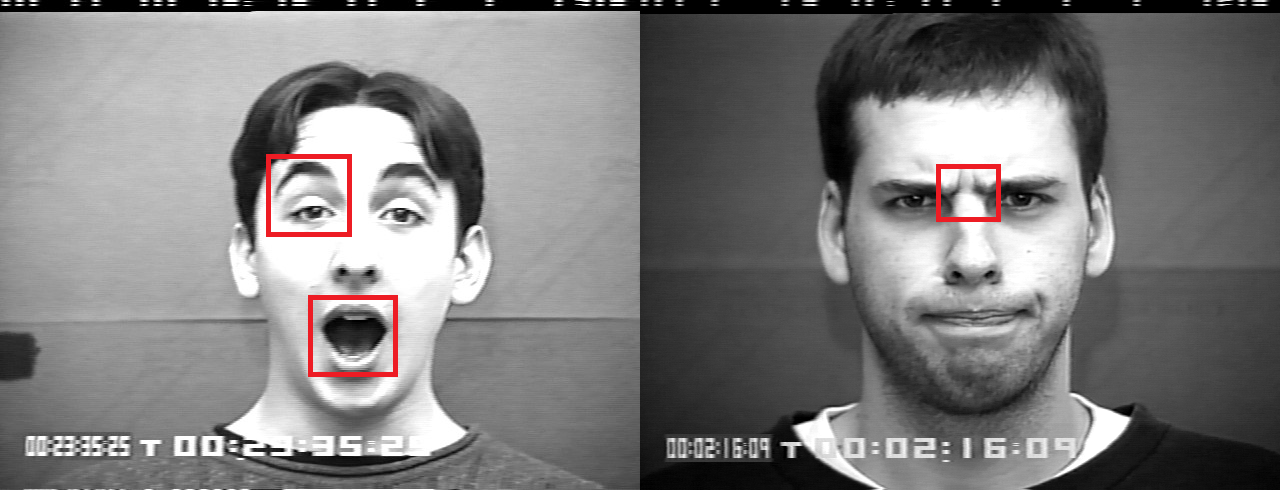
\includegraphics[width=200pt]{img/manual_patch.png}
  \caption{Noticeably discriminating patches}
  \label{fig:manual_patch}
\end{figure}

<<<<<<< Updated upstream
We extracted them manually and rescaled them to 36*36 pixels, 64*64 pixels and 96*96 pixels. Tables \ref{table:left_eye}, \ref{table:right_eye}, \ref{table:between_eyes} and \ref{table:mouth} show the results for each region, for classifiers trained  with the  patch size of 96*96 , 32*32 and 64*64 pixels. Shrinking the images on the one hand results in fewer hog features which is likely to reduce the effect of overfitting, on the other hand some visual information may be lost. The table entries represent the fraction of the images of the corresponding expression that were correctly classified, in the 0 to 1 range.

It was ensured that extracted images of same patch are consistent with each other in terms feature content of the patch. For example, in case of mouth patches, it was ensured that the boundaries of the patch touch the edges of lips in all mouth patches.  It is very important that the patches are consistent and optimal otherwise the results can be poor. This is reflected from Table \ref{table:predict_unaliged_surprise} and Table \ref{table:predict_unaliged_fear}.

\begin{table*}
\centering
\newcommand{\tabincell}[2]{\begin{tabular}{@{}#1@{}}#2\end{tabular}}
\caption{Predicting the unaligned patches from surprise emotion}
\label{table:predict_unaliged_surprise}

\begin{tabular}{| c | c | c | c | c |}
\hline
Patches & Mouth & Left-eye  & Right-eye & \tabincell{c}{Part \\ between eyes}  \\
\hline
1 & sadness & disgust & surprise & fear \\
2 & sadness & fear & disgust & fear \\
3 & neutral & surprise & happy & disgust \\
4 & neutral & disgust & happy & surprise \\
5 & disgust & fear & disgust & fear \\
6 & surprise & fear & sadness & disgust \\
7 & surprise & surprise & sadness & disgust \\
8 & disgust & sadness & disgust & fear \\
9 & surprise & angry & surprise & surprise \\
10 & fear & surprise & disgust & surprise \\
11 & surprise & angry & sadness & fear \\
12 & surprise & angry & disgust & disgust \\
13 & fear & surprise & disgust & disgust \\
14 & surprise & fear & surprise & disgust \\
15 & surprise & surprise & fear & fear \\

\hline
\end{tabular}
\end{table*}


\begin{table*}
\centering
\newcommand{\tabincell}[2]{\begin{tabular}{@{}#1@{}}#2\end{tabular}}
\caption{Predicting the unaligned patches from fear emotion}
\label{table:predict_unaliged_fear}

\begin{tabular}{| c | c | c | c | c |}
\hline
Patches & Mouth &  Left-eye  & Right-eye & \tabincell{c}{Part \\ between eyes} \\
\hline
1 & happy & fear & fear & disgust \\
2 & happy & disgust & fear & fear \\
3 & contempt & surprise & contempt & fear \\
4 & contempt & disgust & contempt & disgust \\
5 & fear & disgust & disgust & fear \\
6 & fear & fear & sadness & angry \\
7 & disgust & sadness & sadness & surprise \\
8 & fear & disgust & disgust & angry \\
9 & fear & disgust & disgust & fear \\
10 & fear & surprise & disgust & disgust \\
11 & fear & surprise & surprise & fear \\
12 & contempt & fear & disgust & fear \\
13 & fear & disgust & disgust & surprise \\
14 & contempt & disgust & fear & disgust \\
15 & happy & fear & fear & disgust \\
\hline
\end{tabular}
\end{table*}

=======
We identified four such patches, that 2 patches for eyes and one each for mouth and glabella. We extracted them manually and it was ensured that extracted images of same patch are consistent with each other in terms feature content of the patch. For example, in case of mouth patches, it was ensured that the boundaries of the patch touch the edges of lips in all mouth patches.
>>>>>>> Stashed changes

Tables \ref{table:left_eye}, \ref{table:right_eye}, \ref{table:between_eyes} and \ref{table:mouth} show the ratios of correct detections for eight facial expressions for each region, for classifiers trained
with the original patch size of 96x96 and also rescaled to 32x32 and 64x64 pixels. Shrinking the images on the one hand results in fewer hog features which is likely to reduce the effect of overfitting, on the other hand some visual information may be lost. The table entries represent the fraction of the images of the corresponding expression that were correctly classified, in the 0 to 1 range.




%\subsection{Results}

\begin{table}

    \begin{subtable}[b]{3in}
    \centering
    \begin{tabular}{| c | c | c | c |}
    \hline
    Expression & 32 x 32 &  64 x 64  & 96 x 96  \\
    \hline
    Angry & 0.5865 & 0.6786 & 0.7068 \\
    Contempt & 0.6596 &	0.5745 & 0.5532 \\
    Disgust	& 0.7629 &	0.7629 &	0.7716 \\
    Fear &	0.6155 & 0.6315 & 0.6394 \\
    Happy &	0.6074 & 0.6605 & 0.6529 \\
    Neutral & 0.6851 &	0.6996 & 0.7093 \\
    Sadness & 0.5207 & 0.5041 &	0.5021 \\
    Surprise & 0.7652 &	0.7683 & 0.7561 \\
    \hline
    \end{tabular}
    \caption{Left eye patches}
    \label{table:left eye}
    \end{subtable}
\quad


    \begin{subtable}[b]{3in}
    \centering
    \begin{tabular}{| c | c | c | c |}
    \hline
    Expression & 32 x 32 &  64 x 64  & 96 x 96  \\
    \hline
    Angry    & 0.5733 & 0.6466 & 0.6654 \\
    Contempt & 0.5638 & 0.5106 & 0.6170 \\
    Disgust	 & 0.7263 & 0.7414 & 0.7155 \\
    Fear	 & 0.6474 & 0.6076 & 0.6096 \\
    Happy	 & 0.6367 & 0.6334 & 0.6833 \\
    Neutral  & 0.7099 & 0.7272 & 0.7562 \\
    Sadness  & 0.5000 & 0.5207 & 0.5456 \\
    Surprise & 0.7896 & 0.8171 & 0.8079 \\
    \hline
    \end{tabular}
    \caption{Right eye patches}
    \label{table:right eye}
    \end{subtable}
\quad


    \begin{subtable}[b]{3in}
    \centering
    \begin{tabular}{| c | c | c | c |}
    \hline
    Expression & 32 x 32 &  64 x 64  & 96 x 96  \\
    \hline
    Angry & 0.7971 & 0.812 & 0.7857 \\
    Contempt & 0.4468 & 0.4574 & 0.4681 \\
    Disgust & 0.6983 & 0.7155 & 0.7306 \\
    Fear & 0.7071 & 0.7649 & 0.7351 \\
    Happy & 0.8503 & 0.8503 & 0.8329 \\
    Neutral & 0.7438 & 0.7845 & 0.7921 \\
    Sadness & 0.7324 & 0.7697 & 0.7635 \\
    Surprise & 0.7317 & 0.7485 & 0.7165 \\
    \hline
    \end{tabular}
    \caption{Right eye patches}
    \label{table:between eyes}
    \end{subtable}
\quad


    \begin{subtable}[b]{3in}
    \centering
    \begin{tabular}{| c | c | c | c |}
    \hline
    Expression & 32 x 32 &  64 x 64  & 96 x 96  \\
    \hline
    Angry	&	0.7782	&	0.8064	&	0.7970	\\
    Contempt	&	0.6277	&	0.6598	& 0.6702 \\
    Disgust	&	0.6918	&	0.7953	&	0.8039	\\
    Fear	&	0.7510	&	0.8287	&	0.8307	\\
    Happy	&	0.8959	&	0.9121	&	0.9154	\\
    Neutral	&	0.7974	&	0.8577	&	0.8501	\\
    Sadness	&	0.8589	&	0.8651	&	0.8693	\\
    \hline
    \end{tabular}
    \caption{Mouth patches}
    \label{table:mouth}
    \end{subtable}

\label{table:results of patches}
\caption[Ratios of correct detections for eight facial expressions]{Ratios of correct detections for eight facial expressions. Table \ref{table:left eye}, Table \ref{table:right eye}, Table \ref{table:between eyes} and Table \ref{table:mouth} shows the result of all left-eye patches, all right-eye patches, patches of the part between eyes and all mouth patches respectively. The results of four kind of patches were all based on the sizes of 32x32 pixels, 64x64 pixels and 96x96 pixels.}
\end{table}

\subsection{SVM on the entire facial images}
We also experimented with training SVM classifiers considering the entire facial area as a single patch. First the bounding box of the face was detected
for each image using the Viola-Jones algorithm, then rescaled to a uniform size. % TODO: Add Reference.
The rest of the procedure was identical to the preceding experiment. The results can be found in Table \ref{table:entire_images}.

\begin{table}
\begin{tabular}{| c | c | c | c |}
\hline
Expression & 32 x 32 &  64 x 64  & 96 x 96  \\

\hline
Angry	 & 0.6165 & 0.6316 & 0.6297	\\
Contempt & 0.4894 & 0.5000 & 0.4043	\\
Disgust	 & 0.7109 & 0.8793 & 0.9367	\\
Fear	 & 0.3540 & 0.6574 & 0.6420	\\
Happy	 & 0.8080 & 0.9317 & 0.9360	\\
Neutral	 & 0.7203 & 0.8260 & 0.8225	\\
Sadness	 & 0.5996 & 0.5830 & 0.6432	\\
Surprise & 0.8765 & 0.9405 & 0.9665	\\

\hline
\end{tabular}
\caption{Classifying the whole image}
\label{table:entire_images}
\end{table}


\subsection{Results of Prediction}
After training SVM classifier, we needed to know whether the classifier is able to predict the training data. We picked out all aligned patches (the part between eyes, left eye, right eye and mouth) from one subject with complete time series of almost emotions. As above memtioned, rescaling has no great influence on the results, so we just experimented with all patches with the size of 96x96 pixels.We listed the best classifications the prediction provided of mouth and right-eye patches in the Table \ref{table:predict_mouth} and Table\ref{table:predict_righteye}.
\\
\\
Moreover, we also experimented with some patches from several subjects which were not aligned with training data. These pathes were all from intense expressions of our dataset. The predicted patches were of size 96x96 pixels because rescaling has no effect as mentioned. We experimented with four kind of patches respectively from one emotion and observed how much outputs would match. Table \ref{table:predict_unaliged_surprise} and Table \ref{table:predict_unaliged_fear} listed the results of patches from 15 subjects in the surprise and fear emotions. The results will indicate the effect of alignment of patches.

\begin{table*}
\centering

    \begin{subtable}{4.7in}
    %\centering
    \begin{tabular}{|*{15}{p{1.34cm}<{\centering}|}|}
    \hline
    Time & Angry &  Disgust  & Fear & Happy & Sadness & Surprise  \\
    \hline
    1 & neutral & neutral & neutral & neutral & neutral & neutral \\
    2 & neutral & neutral & neutral & neutral & neutral & neutral \\
    3 & neutral & neutral & neutral & neutral & neutral & neutral \\
    4 & neutral & neutral & neutral & disgust & neutral & neutral \\
    5 & neutral & neutral &neutral & happy & neutral & neutral \\
    6 & neutral & neutral & disgust & happy & neutral & disgust \\
    7 & neutral & disgust & fear & happy & neutral & surprise \\
    8 & neutral & disgust & fear & happy & neutral & surprise \\
    9 & neutral & disgust & fear & happy & sadness & surprise \\
    10 & contempt & disgust & fear & happy & sadness & surprise \\
    11 & neutral & disgust & fear & happy & sadness & surprise \\
    12 & contempt & disgust & fear & happy & sadness & surprise \\
    13 & angry & disgust & fear & happy & sadness & surprise \\
    14 & angry & disgust & fear & happy & sadness & surprise \\
    15 & angry & disgust & fear & happy & sadness & surprise\\
    \hline
    \end{tabular}
    \label{table:predict_mouth}
    \caption{Aligned mouth patches}
    \end{subtable}
\qquad

    \begin{subtable}{4.7in}
    %\centering
    \begin{tabular}{|*{15}{p{1.34cm}<{\centering}|}|}
    \hline
    Time & Angry &  Disgust  & Fear & Happy & Sadness & Surprise  \\
    \hline
    1 & disgust & neutral & neutral & neutral & neutral & neutral \\
    2 & neutral & disgust & neutral & neutral & neutral & neutral \\
    3 & neutral & neutral & neutral & neutral & neutral & neutral \\
    4 & disgust & neutral & neutral & contempt & neutral & neutral \\
    5 & neutral & contempt & neutral & contempt & neutral & neutral	\\
    6 & happy & contempt & neutral & contempt & contempt & neutral \\
    7 & contempt & disgust & neutral & happy & contempt & neutral \\
    8 & neutral & disgust & contempt & happy & neutral & neutral \\
    9 & contempt & disgust & happy & happy & sadness & surprise \\
    10 & contempt & disgust & contempt & happy & sadness & surprise	\\
    11 & contempt & disgust & contempt & happy & sadness & surprise \\
    12 & neutral & disgust & neutral & happy & sadness & surprise \\
    13 & contempt & disgust & contempt & happy & sadness & surprise \\
    14 & contempt & disgust & neutral & happy & sadness & surprise \\
    15 & neutral & disgust & neutral & happy & sadness & surprise\\

    \hline
    \end{tabular}
    \caption{Aligned right-eye patches}
    \label{table:predict_righteye}
    \end{subtable}

\caption[Results of prediction of aligned patches]{Results of prediction of aligned mouth and right-eye patches with time series from all images of one subject. That means each kind of patches was ordered from neutral to intense one. All predicted patches were of size 96x96 pixels. }
\label{table:predict_righteye}
\end{table*}


\begin{table}

    \begin{subtable}{3in}
    \newcommand{\tabincell}[2]{\begin{tabular}{@{}#1@{}}#2\end{tabular}}
    \begin{tabular}{|*{1}{p{0.3cm}<{\centering}|} c | c | c | c |}
    \hline
      & Mouth & Left-eye  & Right-eye & \tabincell{c}{Part \\ between\\ eyes}  \\
    \hline
    1 & sadness & disgust & surprise & fear \\
    2 & sadness & fear & disgust & fear \\
    3 & neutral & surprise & happy & disgust \\
    4 & neutral & disgust & happy & surprise \\
    5 & disgust & fear & disgust & fear \\
    6 & surprise & fear & sadness & disgust \\
    7 & surprise & surprise & sadness & disgust \\
    8 & disgust & sadness & disgust & fear \\
    9 & surprise & angry & surprise & surprise \\
    10 & fear & surprise & disgust & surprise \\
    11 & surprise & angry & sadness & fear \\
    12 & surprise & angry & disgust & disgust \\
    13 & fear & surprise & disgust & disgust \\
    14 & surprise & fear & surprise & disgust \\
    15 & surprise & surprise & fear & fear \\
    \hline
    \end{tabular}
    \caption{Unaligned patches from surprise emotion}
    \label{table:predict_unaliged_surprise}
        \end{subtable}
\qquad

    \begin{subtable}{3in}
    \newcommand{\tabincell}[2]{\begin{tabular}{@{}#1@{}}#2\end{tabular}}
    \begin{tabular}{|*{1}{p{0.3cm}<{\centering}|} c | c | c | c |}
    \hline
      & Mouth &  Left-eye  & Right-eye & \tabincell{c}{Part \\ between\\ eyes} \\
    \hline
    1 & happy & fear & fear & disgust \\
    2 & happy & disgust & fear & fear \\
    3 & contempt & surprise & contempt & fear \\
    4 & contempt & disgust & contempt & disgust \\
    5 & fear & disgust & disgust & fear \\
    6 & fear & fear & sadness & angry \\
    7 & disgust & sadness & sadness & surprise \\
    8 & fear & disgust & disgust & angry \\
    9 & fear & disgust & disgust & fear \\
    10 & fear & surprise & disgust & disgust \\
    11 & fear & surprise & surprise & fear \\
    12 & contempt & fear & disgust & fear \\
    13 & fear & disgust & disgust & surprise \\
    14 & contempt & disgust & fear & disgust \\
    15 & happy & fear & fear & disgust \\
    \hline
    \end{tabular}
    \caption{Unaligned patches from fear emotion}
    \label{table:predict_unaliged_fear}
    \end{subtable}

    \caption[Results of prediction of unaligned patches]{Results of prediction of unaligned patches with size of 96x96 from 15 subjects in the dataset. Table \ref{table:predict_unaliged_surprise} and Table \ref{table:predict_unaliged_fear} shows the outputs of four kind of patches in the surprise and fear emotions}
    \label{table:predict unaliged image}
\end{table}
